\documentclass[psamsfonts]{amsart}

%-------Packages---------
\usepackage{amssymb,amsfonts}
\usepackage[all,arc]{xy}
\usepackage{enumerate}
\usepackage{mathrsfs}
\usepackage{subcaption}
\usepackage{graphicx}
\usepackage{caption}


%--------Theorem Environments--------
%theoremstyle{plain} --- default
\newtheorem{thm}{Theorem}[section]
\newtheorem{cor}[thm]{Corollary}
\newtheorem{prop}[thm]{Proposition}
\newtheorem{lem}[thm]{Lemma}
\newtheorem{conj}[thm]{Conjecture}
\newtheorem{quest}[thm]{Question}

\theoremstyle{definition}
\newtheorem{defn}[thm]{Definition}
\newtheorem{defns}[thm]{Definitions}
\newtheorem{con}[thm]{Construction}
\newtheorem{exmp}[thm]{Example}
\newtheorem{exmps}[thm]{Examples}
\newtheorem{notn}[thm]{Notation}
\newtheorem{notns}[thm]{Notations}
\newtheorem{addm}[thm]{Addendum}
\newtheorem{exer}[thm]{Exercise}

\theoremstyle{remark}
\newtheorem{rem}[thm]{Remark}
\newtheorem{rems}[thm]{Remarks}
\newtheorem{warn}[thm]{Warning}
\newtheorem{sch}[thm]{Scholium}

\makeatletter
\let\c@equation\c@thm
\makeatother
\numberwithin{equation}{section}

\bibliographystyle{plain}

%--------Meta Data: Fill in your info------
\title{Problem Set 1 \\ 6.864}

\author{Won I. Lee}

%\date{July 30, 2016}


\begin{document}
	
\maketitle

\section{Smoothing}

\subsection{} Note that the log-likelihood of the training corpus (size $N$) is given by:
$$\log P(w_1, \dots, w_N) = \sum_{i=1}^N \log P(w_i|w_{i-1}, w_{i-2}) = \sum_{i=1}^N \log\left(\frac{\text{count}(w_{i-2}, w_{i-1}, w_i) + \alpha}{\text{count}(w_{i-2}, w_{i-1}) + \alpha |V|}\right)$$
Thus, as $\alpha\rightarrow\infty$, the terms all go to $1/|V|$, as the smoothing term dominates the count terms. In this case we end up with a log-likelihood of $-N\log|V|$. Note that with $\alpha = 0$, we have the MLE estimate, so that the log-likelihood of the training corpus must be greatest at that $\alpha = 0$. Thus, we expect a decline in log-likelihood starting from the MLE value at $\alpha = 0$ to the limiting value of $-N\log|V|$ as $\alpha \rightarrow \infty$, as sketched in {\bf Figure 1}.

\begin{figure}
	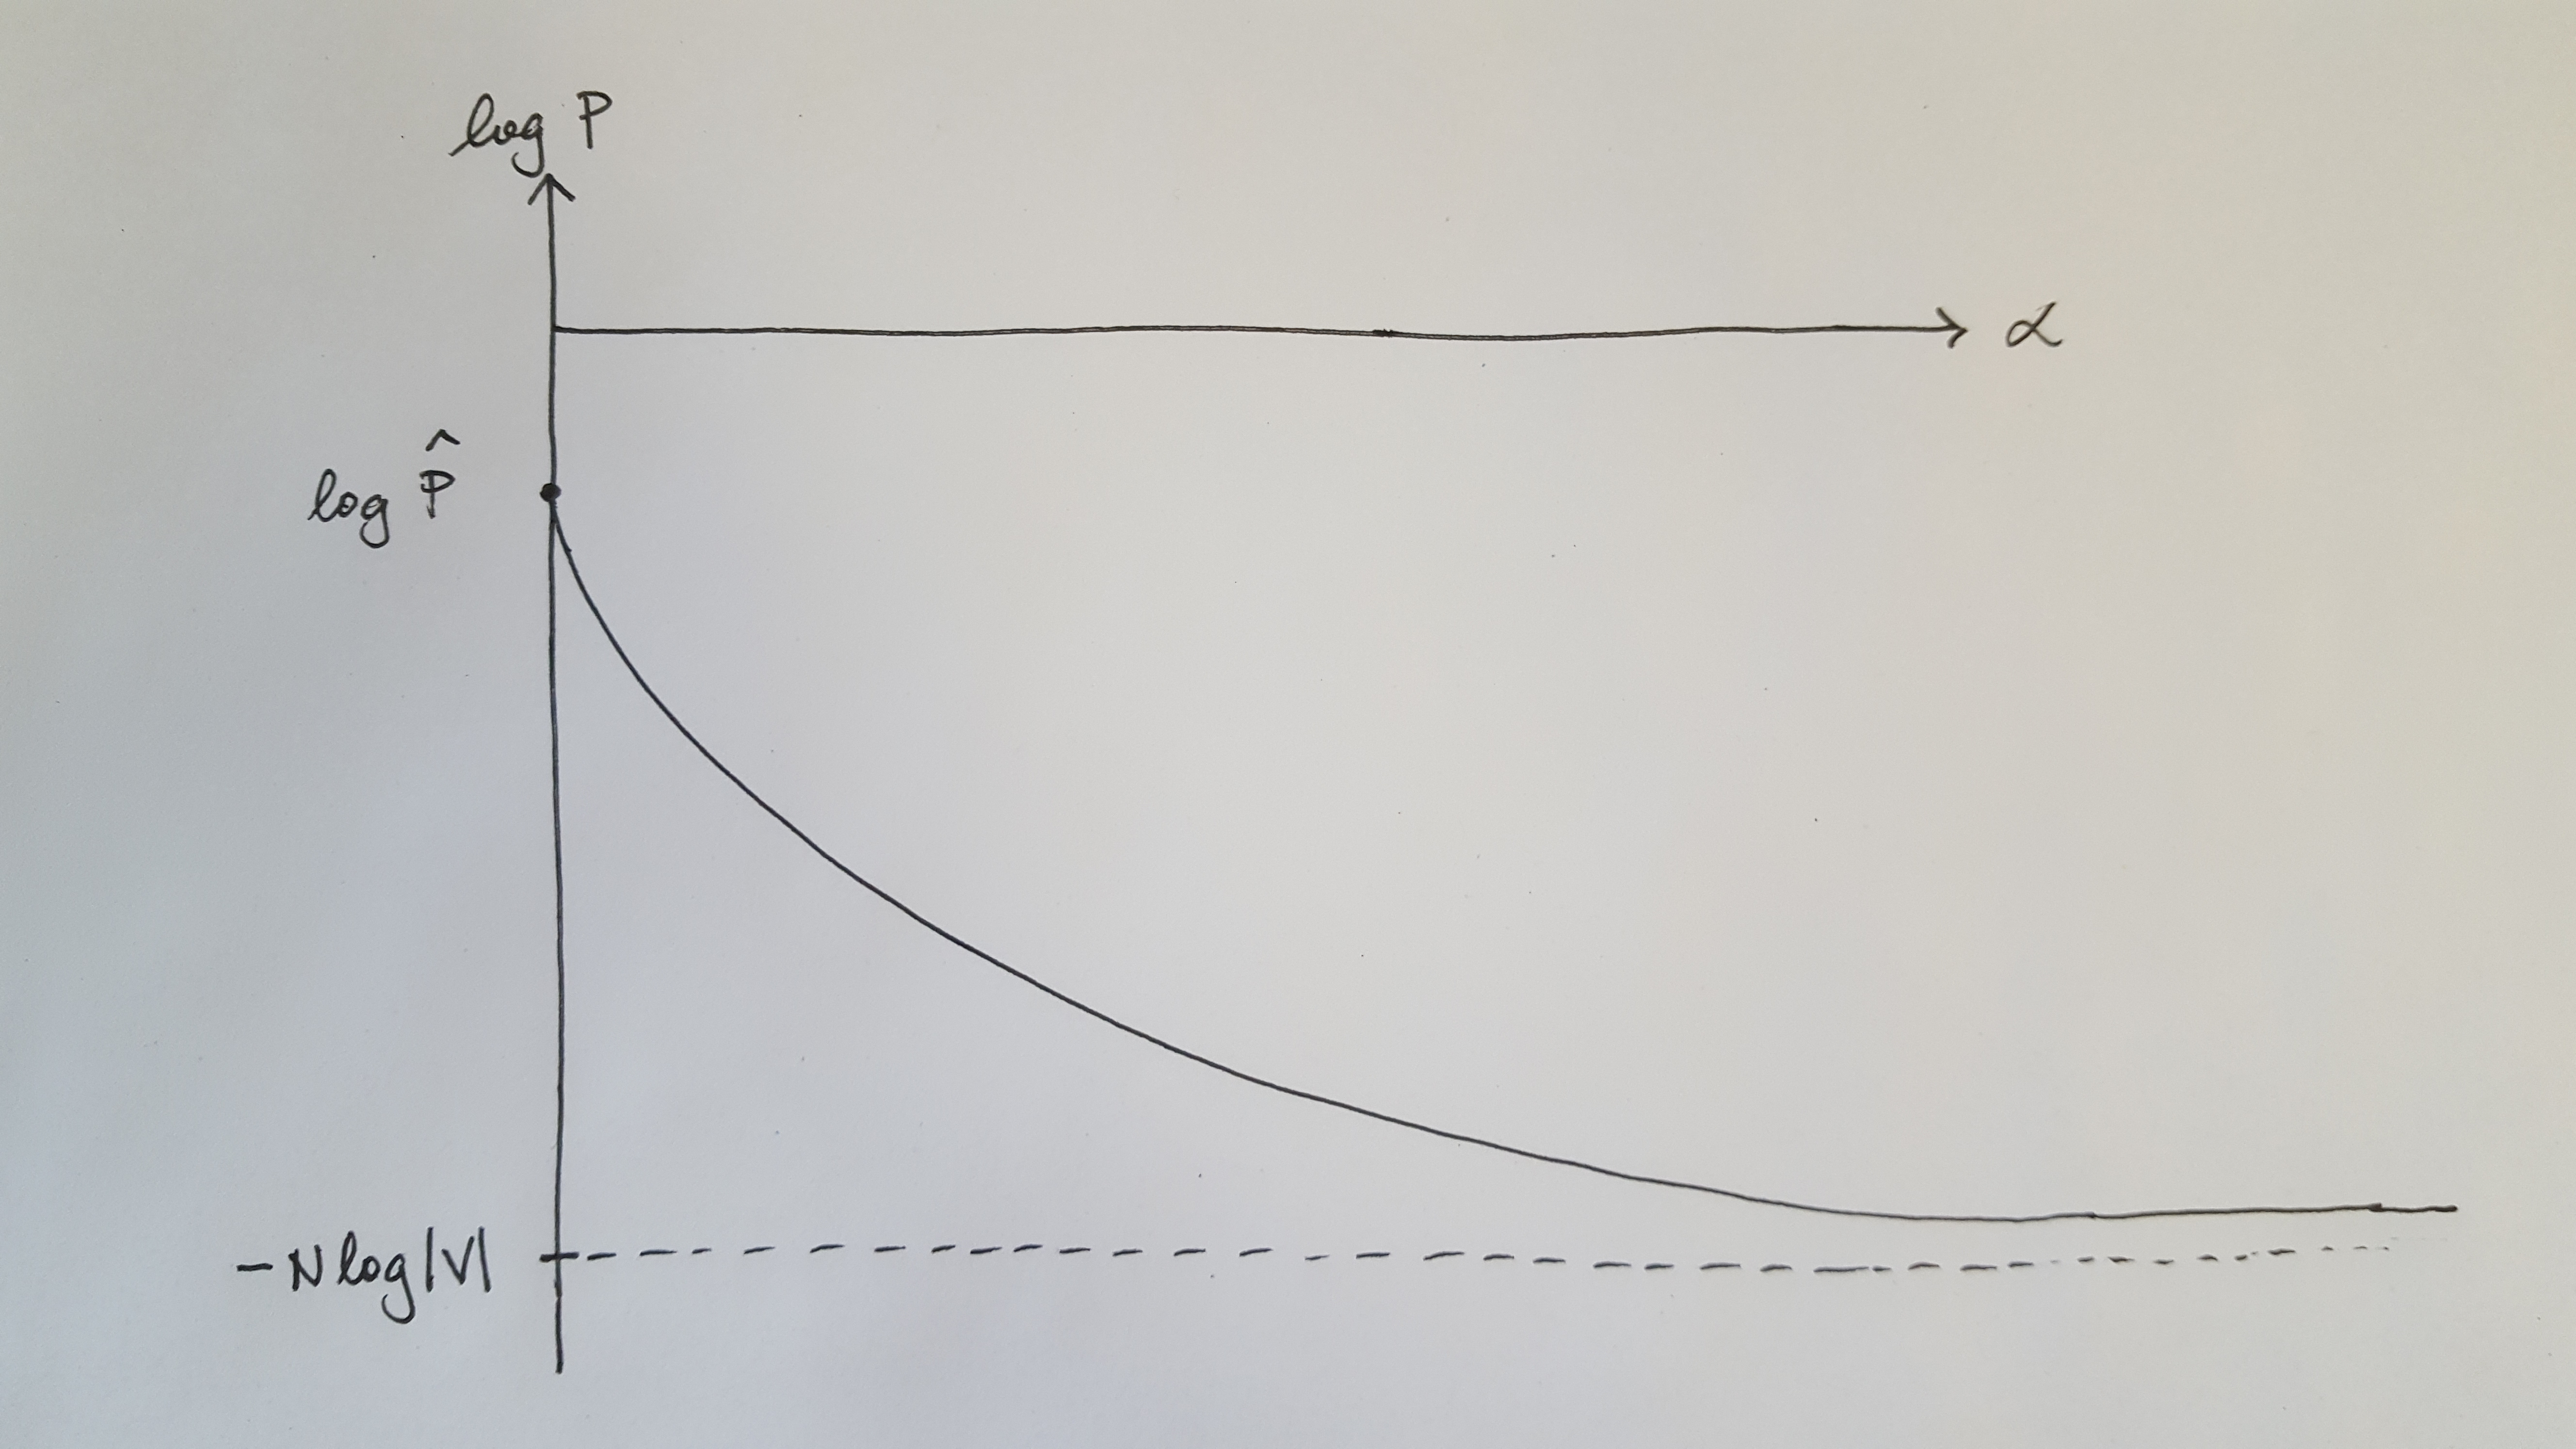
\includegraphics[width=0.6\textwidth]{1-1.jpg}
	\caption{Sketch of log-likelihood of training corpus.}
\end{figure}

\subsection{} On a large test corpus, there will almost surely be a tri-gram that is not seen in the training corpus. Thus, for this tri-gram, $p(w_t|w_{t-2},w_{t-1}) = 0$ with no smoothing, so the log-likelihood of the test corpus will be $-\infty$ with $\alpha = 0$.

Given the non-trivial performance of tri-gram models in practice, it is also likely that for some smoothing factor $0 <\alpha < \infty$, the log-likelihood will be greater (i.e. model performs better) than that of a uniform uni-gram model, which is what the $\alpha\rightarrow\infty$ limit represents. Thus, for some values of $\alpha$, we must have $\log P(w_1, \dots, w_N) > -N\log|V|$, where $N$ is now the size of the test corpus, and so a curve such as in {\bf Figure 2} may result.

\begin{figure}
	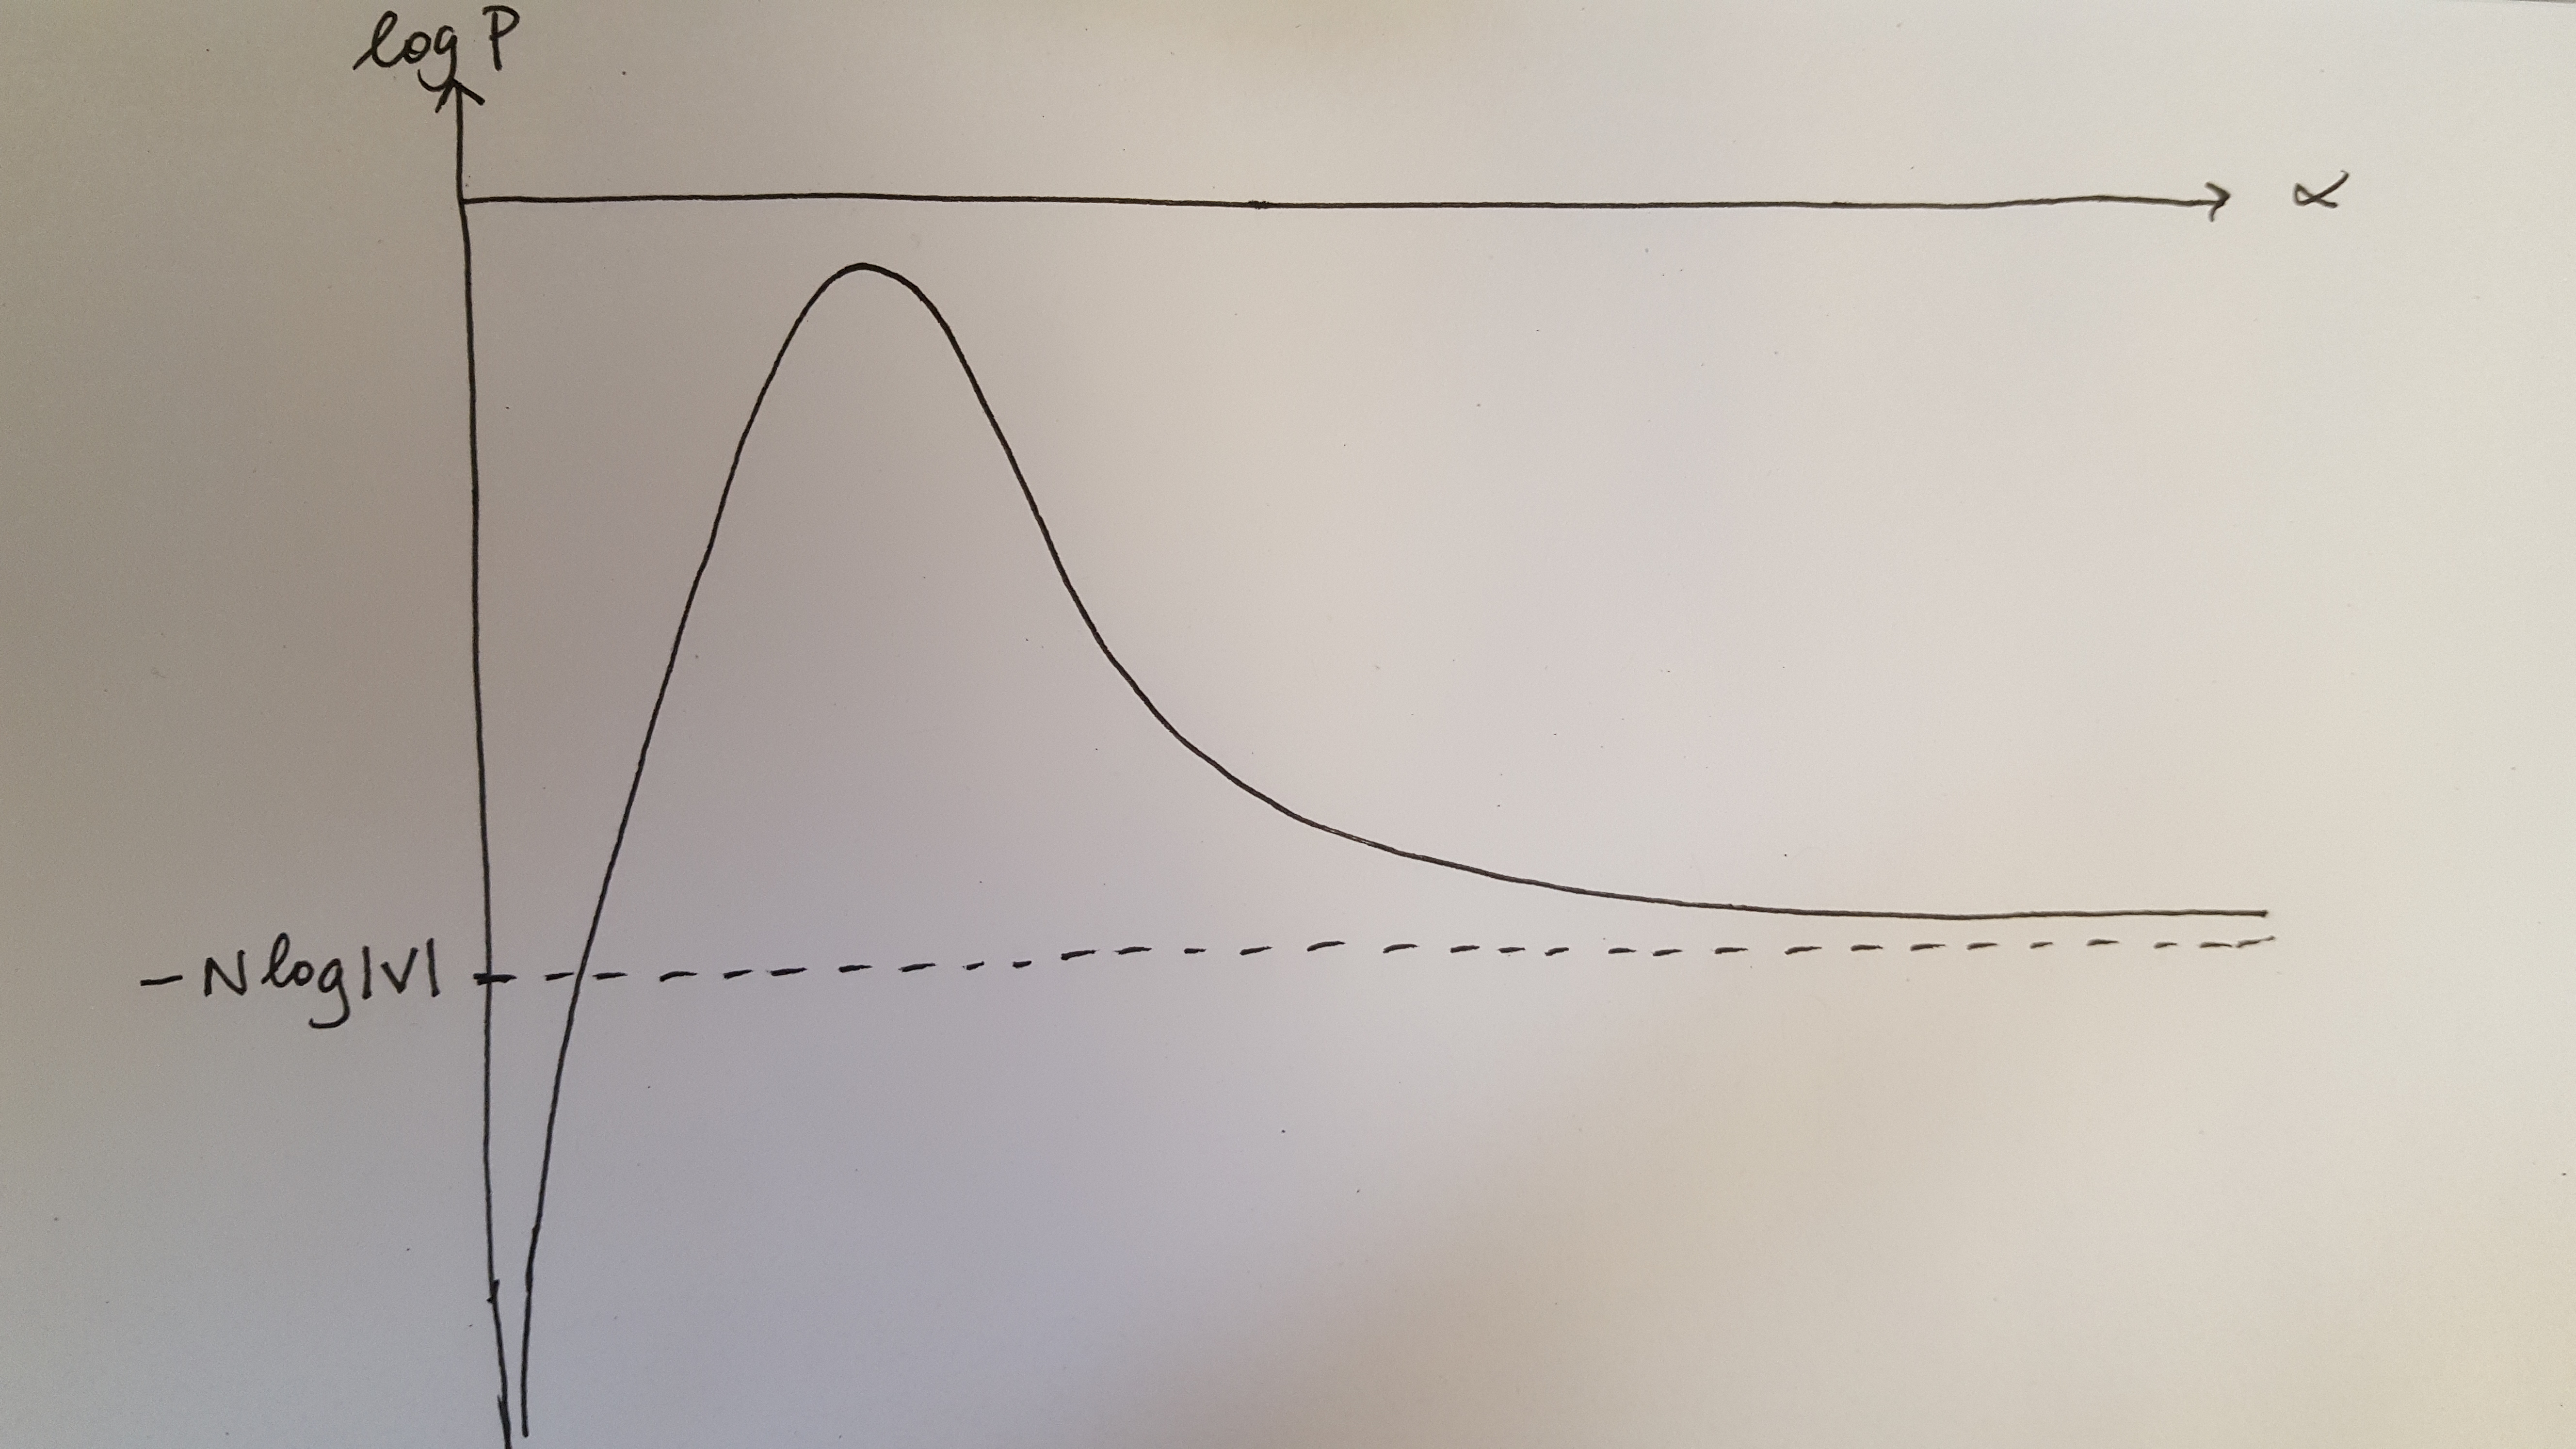
\includegraphics[width=0.6\textwidth]{1-2.jpg}
	\caption{Sketch of log-likelihood of test corpus.}
\end{figure}


\subsection{} The perplexity is simply:
$$\text{perp} = 2^{-\frac{1}{N} \log P(w_1, \dots, w_N)}$$
so as $\alpha \rightarrow\infty$ and $P(w_1, \dots, w_N) \rightarrow -N\log |V|$, $\text{perp} \rightarrow |V|$ is the limiting value. But when $\alpha = 0$, we had a $-\infty$ log-likelihood, which yields $\text{perp} = \infty$. Thus, we expect the perplexity value to behave as in {\bf Figure 3} as $\alpha$ varies, achieving a lower perplexity than a uniform uni-gram model with some non-zero smoothing factor.

\begin{figure}
	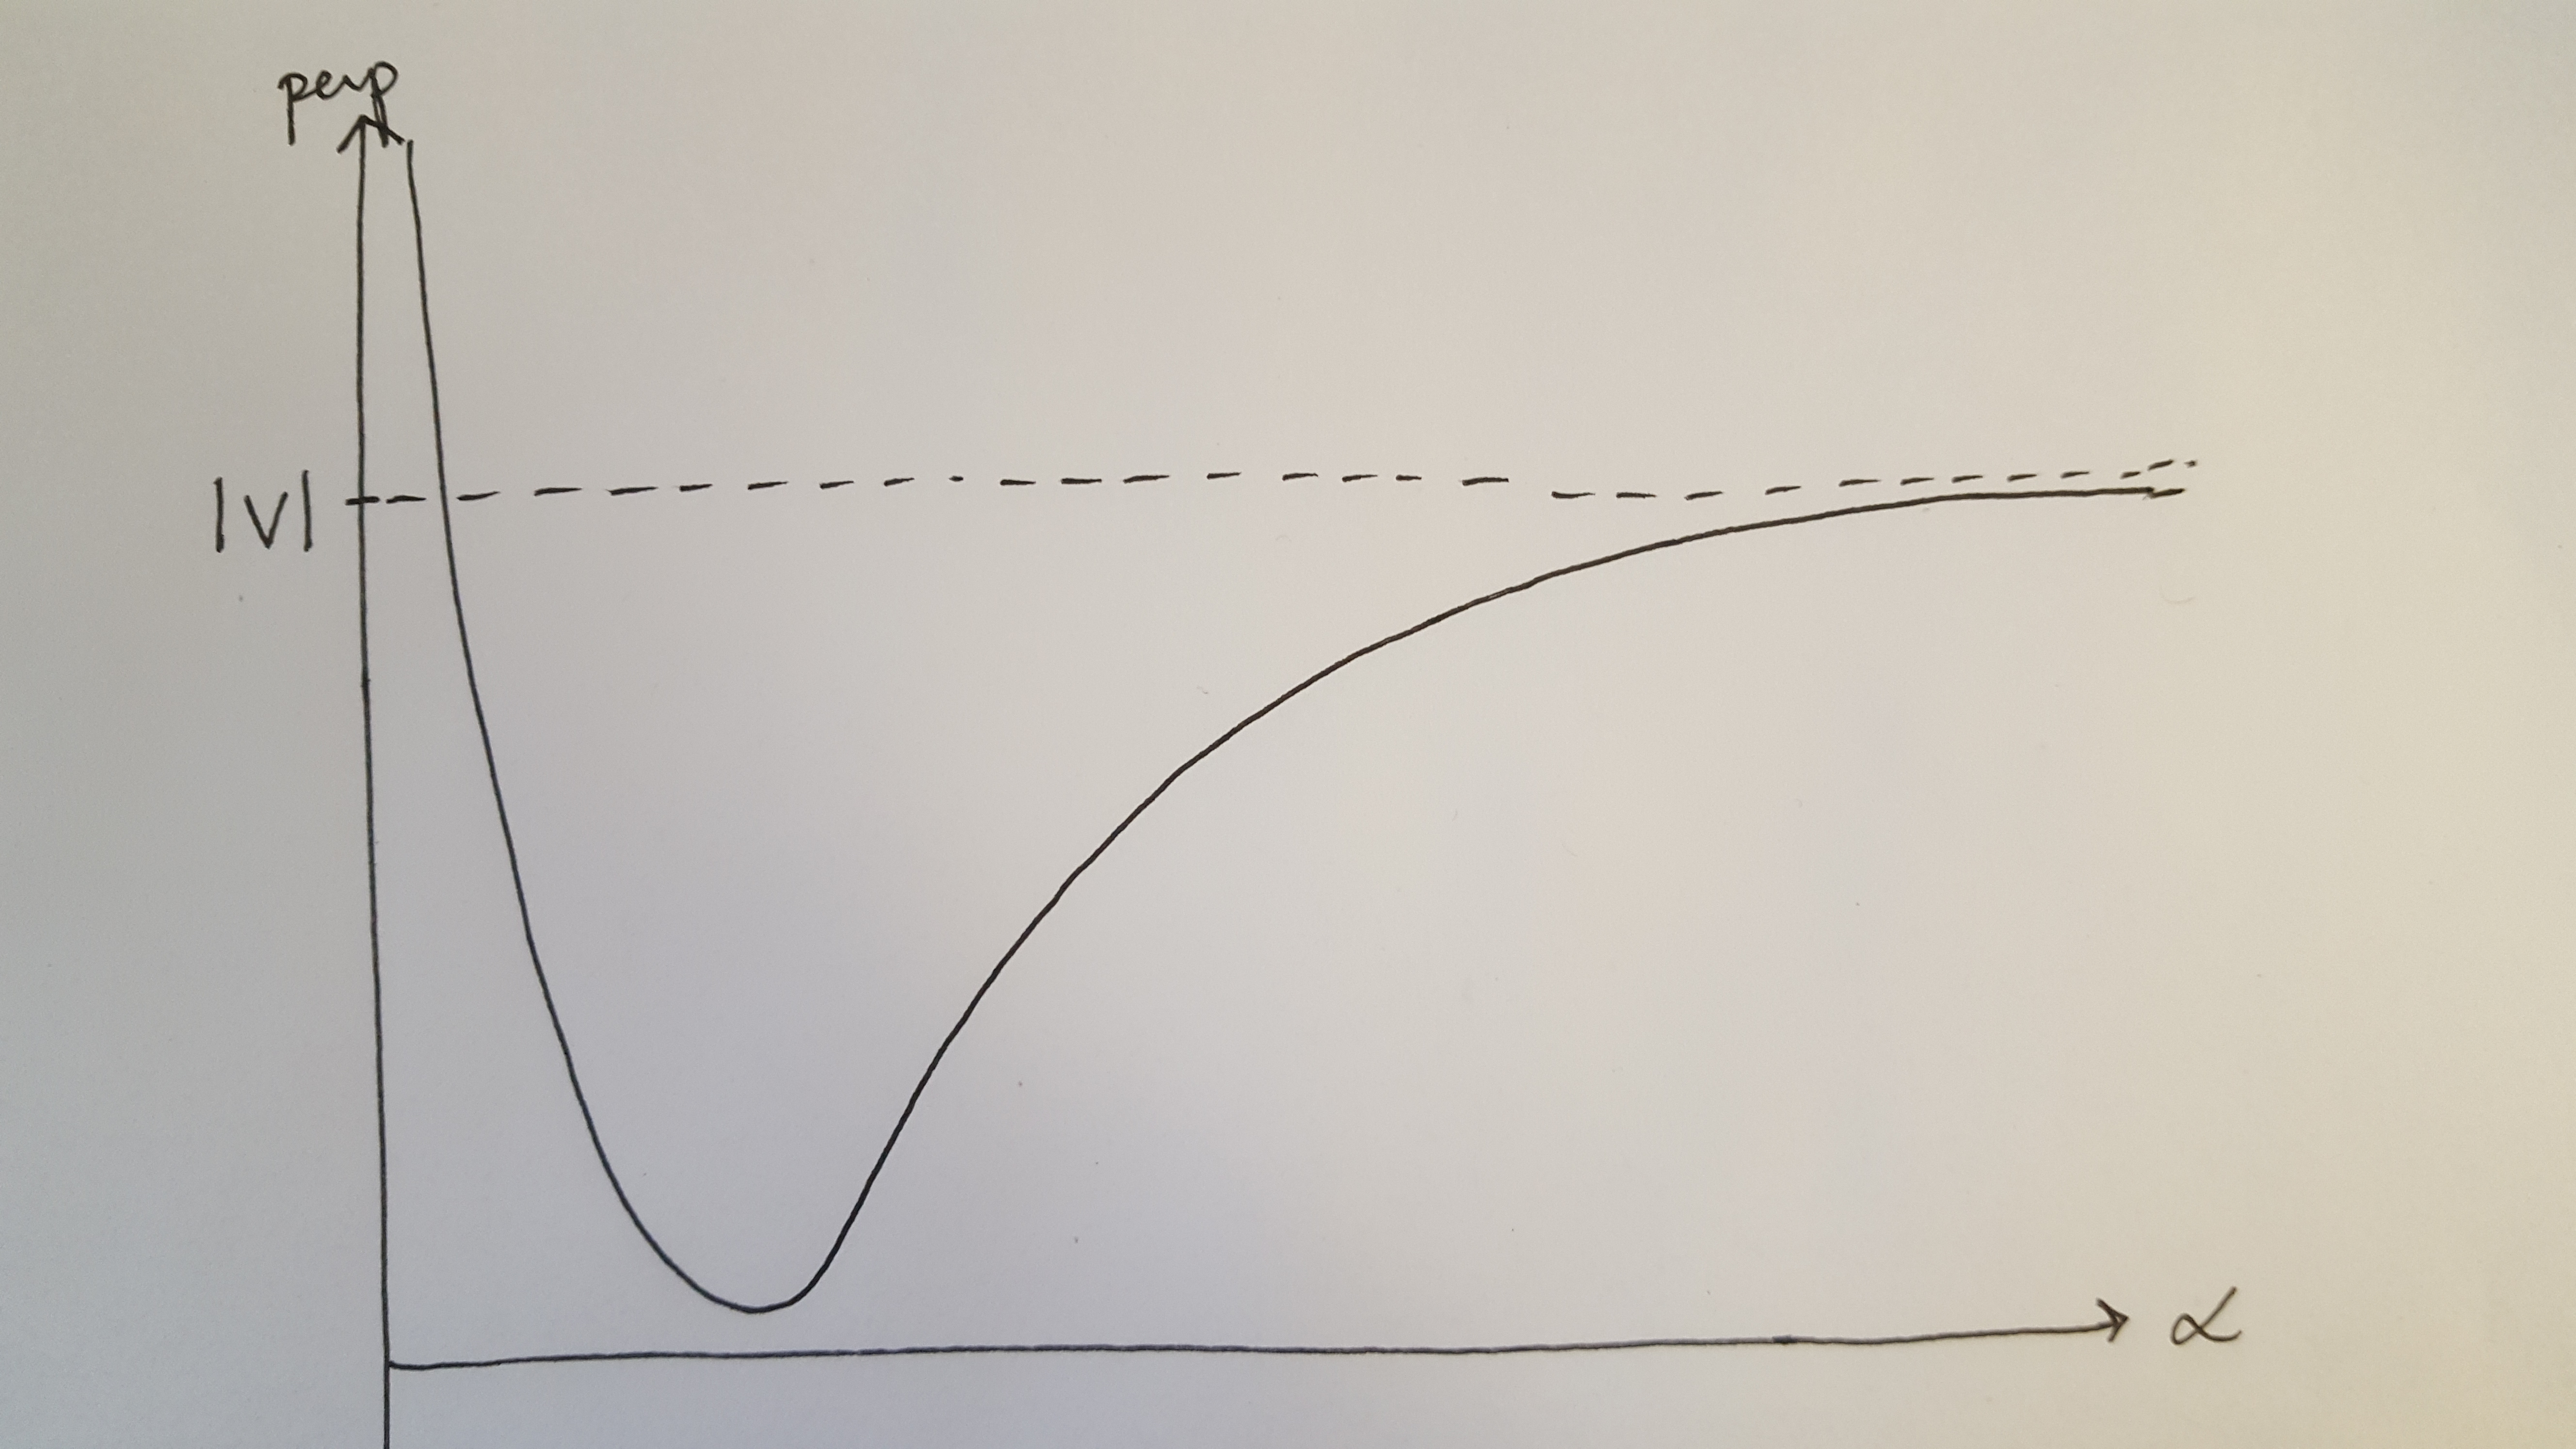
\includegraphics[width=0.6\textwidth]{1-3.jpg}
	\caption{Sketch of perplexity of test corpus.}
\end{figure}

\subsection{} As $\alpha \rightarrow \infty$, we have for any tri-gram:
$$p(w_t|w_{t-2},w_{t-1}) \rightarrow \frac{1}{|V|}$$
since the counts are dominated by the smoothing factor. Thus, the perplexity on the test set becomes:
$$2^{-\frac{1}{L}\log P(w_1, \dots, w_L)} = 2^{-\frac{1}{L}\sum_{i=1}^L \log P(w_i|w_{i-1},w_{i-2})} \rightarrow 2^{-\frac{1}{L}\cdot L \log(1/|V|)} = |V|$$

\section{Neural Language Models}

\subsection{} The concatenated input vector for an $n$-gram has dimension $(n-1)d$, so the input signal computation would require $O(nd)$ computations for each hidden unit, or $O(mnd)$ for the entire signal. Since $\tanh$ takes a constant time per input, the hidden unit activations require $O(m)$ operations. Similarly to before, we require $O(m)$ computations for each input signal, so $O(|V|m)$ overall for the input signal to output. Finally, we can compute the softmax partition function once for all evaluations, requiring $O(|V|)$ computations, and then evaluate the entire softmax distribution using another $O(|V|)$ operations, so the softmax step takes $O(|V|)$ overall. Thus, the complexity is:
$$O(mnd + |V|m)$$
assuming that $nd, m \geq 1$.

\subsection{} For a GPU-optimized model, the calculations above are altered so that the input signal to hidden units requires only $O(nd)$, hidden unit requires $O(1)$, input signal to output requires $O(m)$, and softmax requires $O(|V|)$, simply to calculate the partition function. Thus, the complexity is:
$$O(nd + m + |V|)$$

\subsection{} We denote $p_y \equiv P(w_t = y|w_{t-1}, w_{t-2})$ for all cases. We start by considering:
$$\frac{\partial \log p_y}{\partial z_{k}^o} = \frac{\partial}{\partial z_k^o} \frac{e^{z_y^o}}{\sum_l e^{z_l^o}} = \left\{ \begin{matrix} \frac{e^{z_y^o}\left( \sum_l e^{z_l^o} - e^{z_k^o} \right)}{\left(\sum_l e^{z_l^o} \right)^2} = p_y^o(1-p_k^o) & y = k \\ -\frac{e^{z_y^o}e^{z_k^o}}{\left(\sum_l e^{z_l^o} \right)^2} = -p_y^o p_k^o & y \neq k \end{matrix} \right.$$
Thus, we have:
$$\delta_k^o = \frac{\partial \log p_y}{\partial z_k^o} = \frac{1}{p_y} \frac{\partial p_y}{\partial z_k^o} = \left\{ \begin{matrix} 1-p_k^o & y = k \\ -p_k^o & y\neq k \end{matrix} \right.$$

Now for $\delta_j^h$, we use the chain rule to obtain:

$$\delta_j^h \equiv \frac{\partial \log p_y}{\partial z_j^h} = \sum_k \frac{\partial \log p_y}{\partial z_k^o} \frac{\partial z_k^o}{\partial z_j^h} = \sum_k \delta_k^o \left[ \sum_l \frac{\partial z_k^o}{\partial f_l^h}\frac{\partial f_l^h}{\partial z_j^h} \right]$$
but we have $\frac{\partial z_k^o}{\partial f_l^h} = W_{lk}^o$ and:
$$\frac{\partial f_l^h}{\partial z_j^h} = \left\{ \begin{matrix} 0 & l \neq j \\ \frac{\partial \tanh(z_j^h)}{\partial z_j^h} = 1-\tanh^2(z_j^h) & l = j \end{matrix} \right.$$
Putting these together:
$$\delta_j^h = \sum_j W_{jk}^o (1-\tanh^2(z_j^h)) \delta_k^o$$

Finally, we have:
$$\delta_i^x = \sum_j \frac{\partial \log p_y}{\partial z_j^h}\frac{\partial z_j^h}{\partial x_i} = \sum_j W_{ij}^h\delta_j^h$$

Using $\delta_i^x$, the stochastic gradient step for updating $v(w_{t-2})$ is:
$$v(w_{t-2}) \leftarrow v(w_{t-2}) - \eta \nabla_{x} \log p_y[1:d] = v(w_{t-2}) - \eta (\delta_1^x, \dots, \delta_d^x)$$
where the $[1:d]$ notation represents taking the first $d$ elements of the gradient vector. 

\subsection{} (a) The bi-gram model scored an average test log-likelihood of $-4.96$. On the other hand, using the best configuration of parameters (as reported below), we achieved an average test log-likelihood of $-4.618$.

(b) We tested every combination for a number of different parameter values. Namely, we considered: $n = 2, 3, 5$; $d = 5, 10, 20$; and $m = 10, 30, 50$. We found that the best configuration in terms of development log-likelihood was $n=3, d = 5, m = 50$. The average test log-likelihood for these parameters was, as noted, was $-4.618$.

(c) In {\bf Figure 4} and {\bf Figure 5}, we plot the dependence of the average log-likelihood on both the training set (4) and test set (5), where the legend depicts the word embedding dimension $d$ (i.e. $d = 5, 10, 20$). What is notable is that the average log-likelihood increases monotonically with $m$ on the training set, but decreases after a suitable value on the test set. This is because when $m$ increases, we have more parameters that we can fit, so that the model fits the training set better; but after a certain point, it begins to overfit to the training data. This is evident in Figure 5, where, for example $n = 3$, the average log-likelihood peaks at $ m = 30$ for all values of $d$, and declines afterward due to overfitting issues.

Using the performance on the development set, which the model has not seen, in order to select the ``best" model helps to control for these issues. As visible in Figure 5, by selecting $n=3, d= 5, m = 50$, we actually do not end up choosing the model with the best average log-likelihood on the test set (as we evaluated on the development set), but the results on the test set are very close.

\begin{figure}
	\begin{subfigure}[b]{0.3\textwidth}
		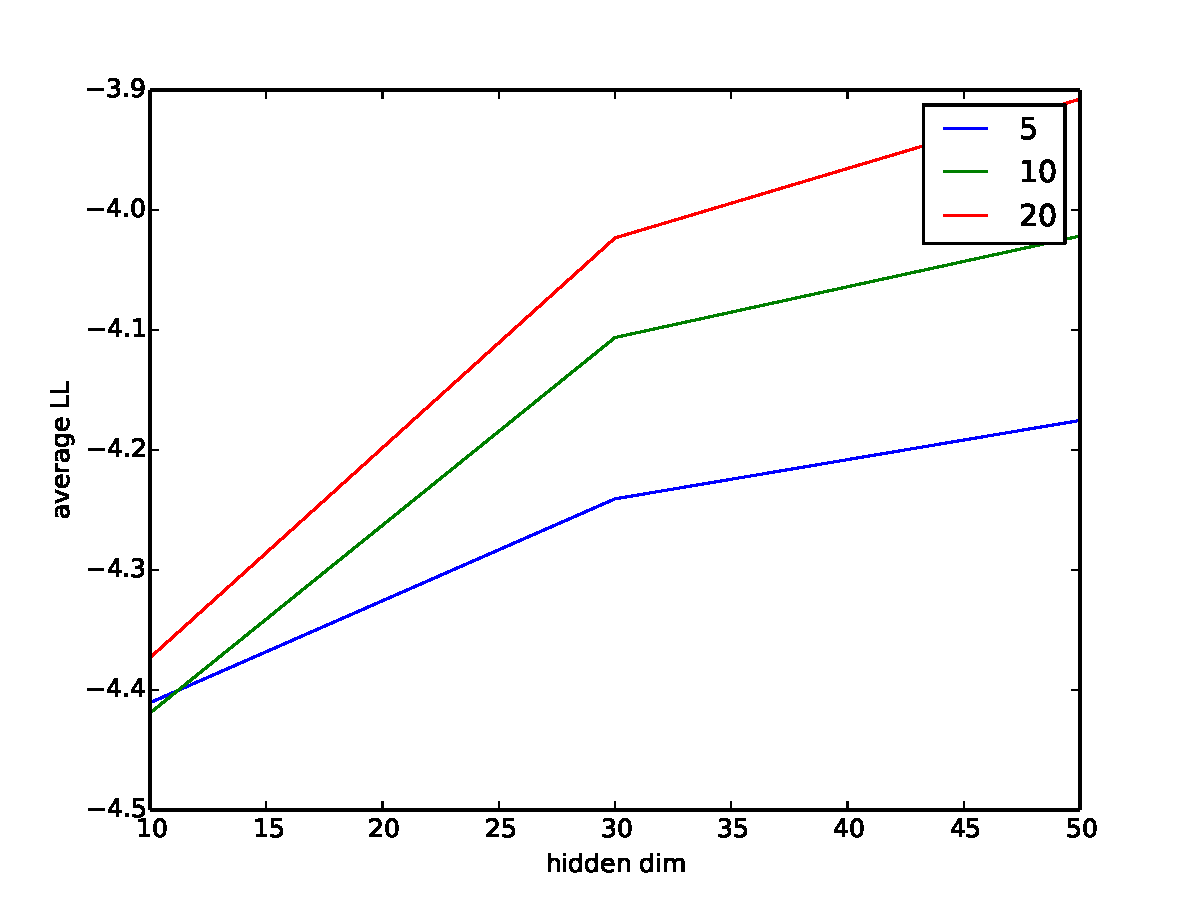
\includegraphics[width=\textwidth]{code/hw1_train_n2.pdf}
		\caption{$n=2$}
	\end{subfigure}
	\begin{subfigure}[b]{0.3\textwidth}
		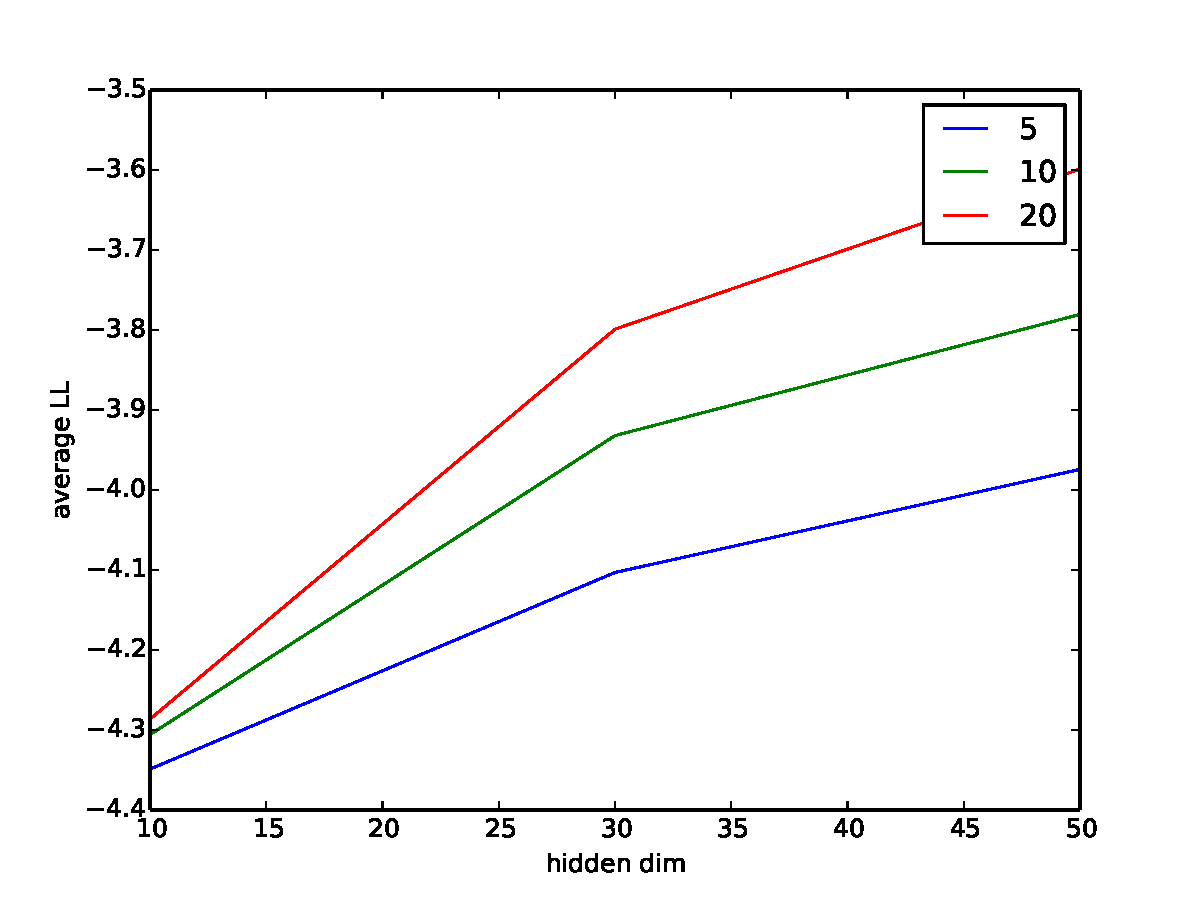
\includegraphics[width=\textwidth]{code/hw1_train_n3.pdf}
		\caption{$n=3$}
	\end{subfigure}
	\begin{subfigure}[b]{0.3\textwidth}
		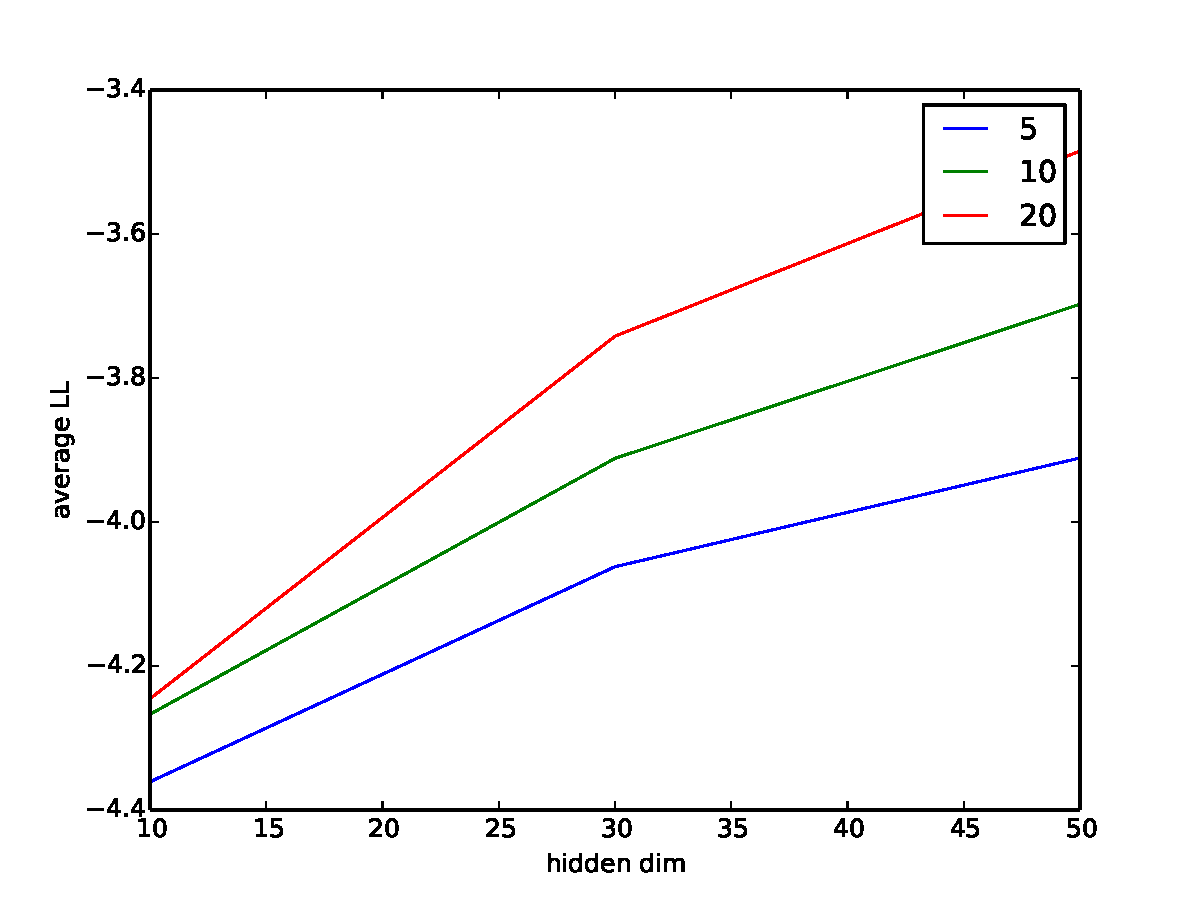
\includegraphics[width=\textwidth]{code/hw1_train_n5.pdf}
		\caption{$n=5$}
	\end{subfigure}
	\caption{Average log-likelihood on training set as a function of $m$ for different configurations.}
\end{figure}

\begin{figure}
	\begin{subfigure}[b]{0.3\textwidth}
		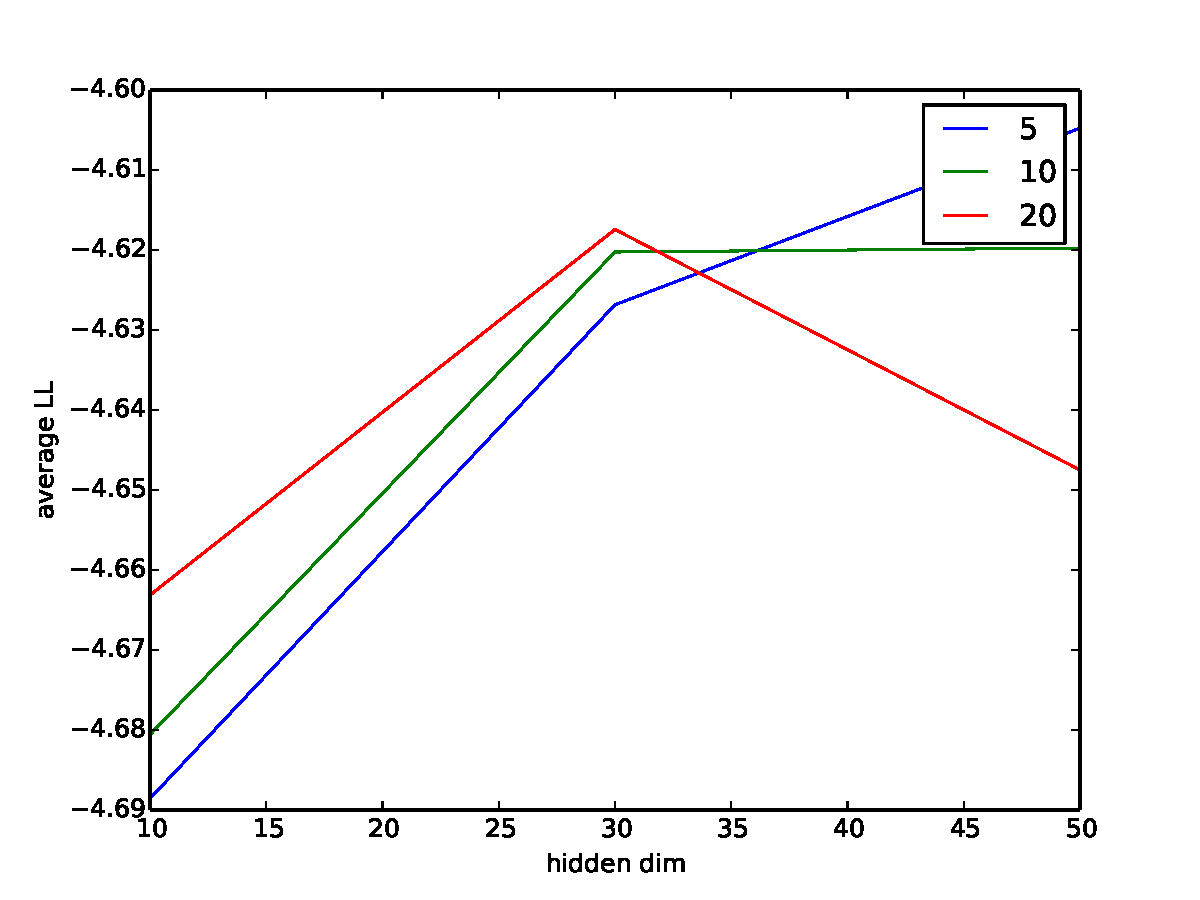
\includegraphics[width=\textwidth]{code/hw1_test_n2.pdf}
		\caption{$n=2$}
	\end{subfigure}
	\begin{subfigure}[b]{0.3\textwidth}
		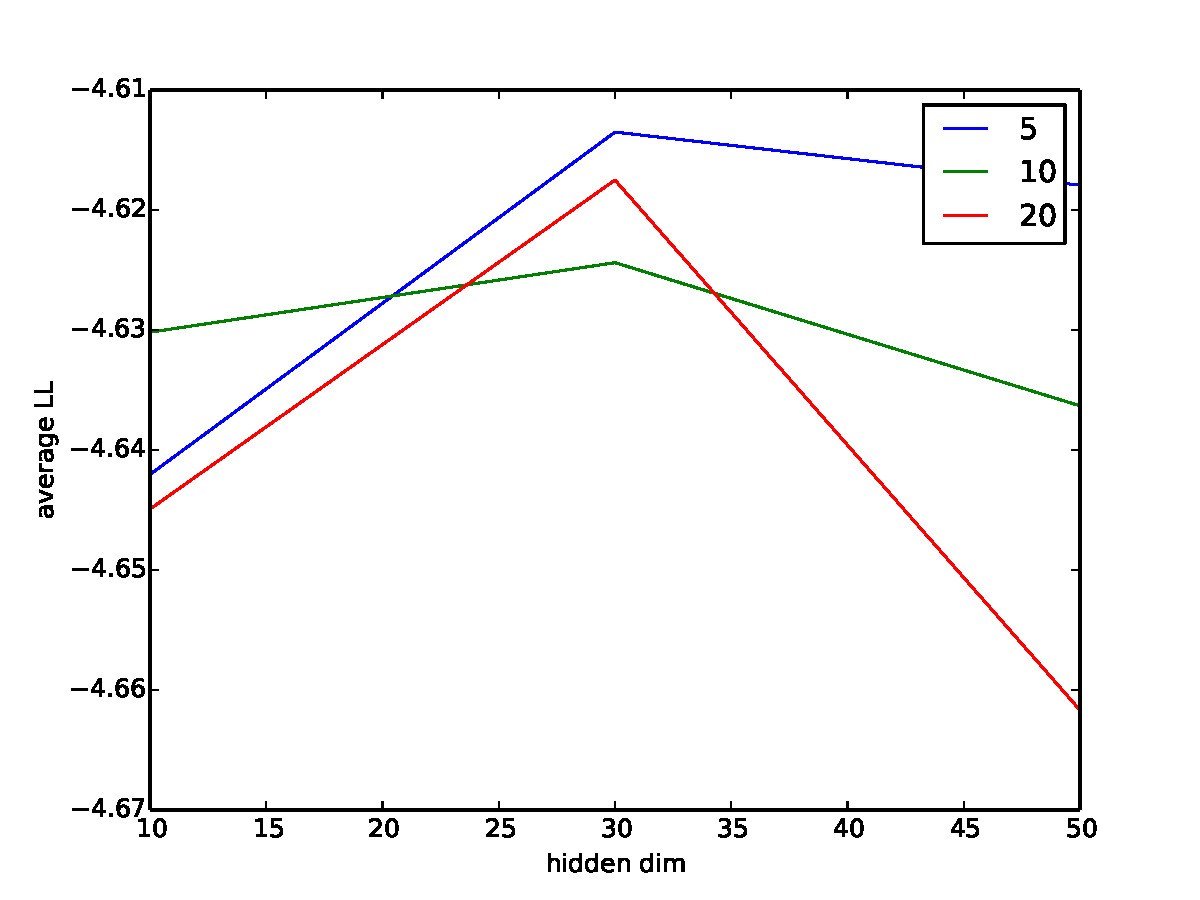
\includegraphics[width=\textwidth]{code/hw1_test_n3.pdf}
		\caption{$n=3$}
	\end{subfigure}
	\begin{subfigure}[b]{0.3\textwidth}
		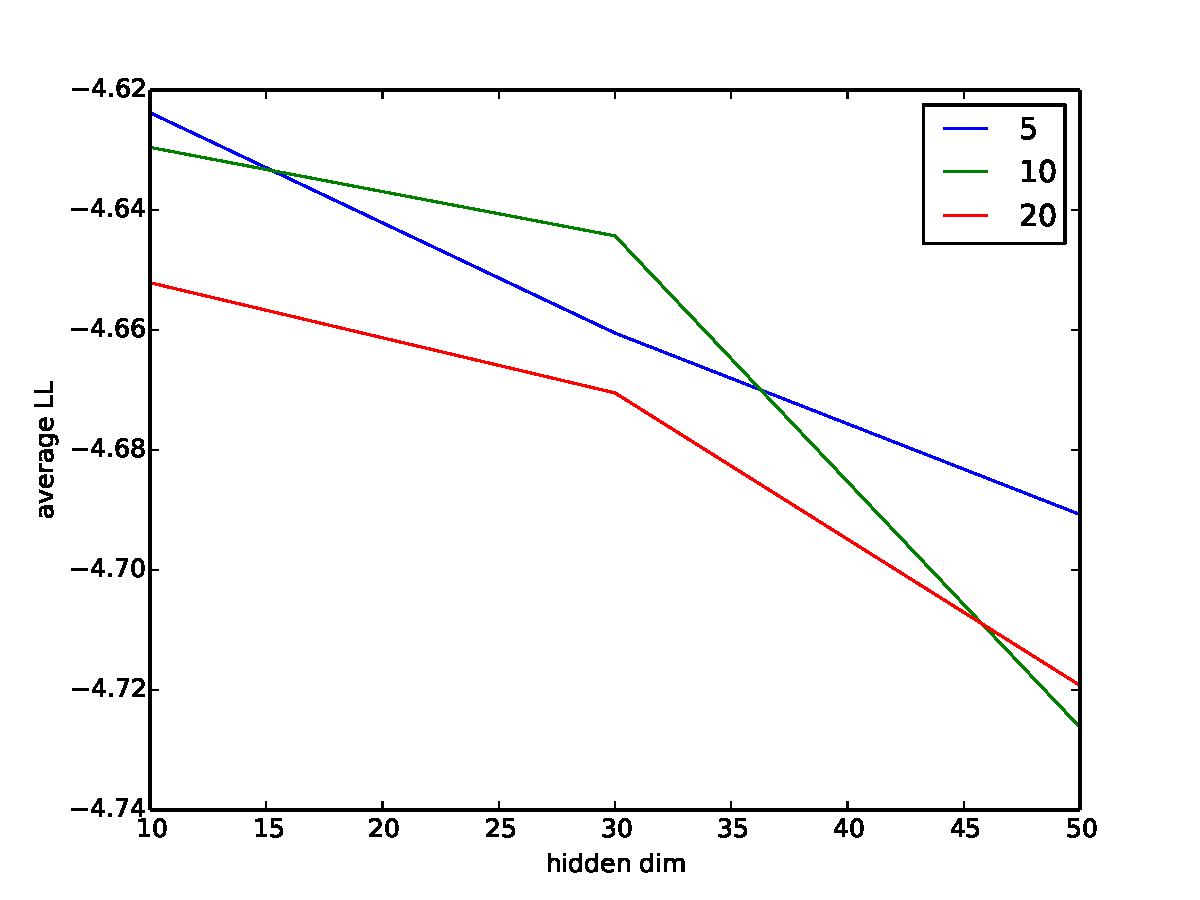
\includegraphics[width=\textwidth]{code/hw1_test_n5.pdf}
		\caption{$n=5$}
	\end{subfigure}
	\caption{Average log-likelihood on test set as a function of $m$ for different configurations.}
\end{figure}

\subsection{} (a) The neural network model will {\bf not} necessarily assign a zero/near-zero value to unseen words. This is because the embedding layer $v(w_{t})$ embeds the words, even unseen words, into a lower-dimensional (as opposed to one-hot) and dense vector. If an unseen word (or $n$-gram) is close in the dense space to another word which has been seen, it will have relatively close probability values to the seen word (i.e. non-zero). However, if the word is unseen, then the embedding vector is completely untrained, so that the embedding is most likely meaningless and distant from learned embeddings. In this case, the model will likely assign a near-zero probability to the unseen word (but as noted above, this need not be the case).

(b) In a similar fashion, the model can assign a reasonable prediction for $w_t$, even if the specific preceding context did not appear in the training set. If the individual words $w_{t-i}$ were seen in training, then the embedding vectors $v(w_{t-i})$ will be trained, so the entire concatenation of vectors $[v(w_{t-1}) \cdots v(w_{t-n+1})]$ will have a reasonable value in the dense embedding space. Thus, a reasonable prediction for $w_t$ can be made in this situation.

\subsection{} We again used the configuration $n=3, d = 5, m = 50$ on this task. We found that the trained model yielded an overall log-likelihood of $-35.06$ (i.e. average log-likelihood of $-4.38$) on the correct example, and $-43.36$ (average log-likelihood of $5.42$) on the incorrect example, so the correct example is more likely according to our model.

\section{Recurrent Neural Language Models}

\subsection{} No. In order to generate the above example sequence with high probability, we must set the parameters such that $P(very|very) \approx 1$ for time steps $t = 4, 5$. However, this precludes our ability to set $P(cool|very) \approx 1$, since the input to the network is identical in both cases (``very''). Thus, without the context $h^{t-1}$, we cannot generate such a sequence with arbitrarily high probability.

\subsection{} Yes. Suppose that we have exactly $8$ hidden units, each essentially being a one-hot vector for each token in the sequence, including start and end tokens. We also have one additional hidden unit that simply records whether the previous word was ``very''. By setting the weights properly, we can then create a deterministic mapping from each word to the next (i.e. by setting the output layer weight $w_{very|always} = 1$ and 0 elsewhere) that yields probability 1 to the example sequence. We can then use the additional hidden unit to make sure that the probability of ``cool'' given ``very, very'' is 1, i.e. by setting $w_{very|very} = 1$ but $w_{very|very(prev)} = -1$ and $w_{always|very(prev)} = 1$.


\end{document}


